% Corrected C1 day-ahead schedule and nominal power balance.
\begin{figure}[t]
  \centering
  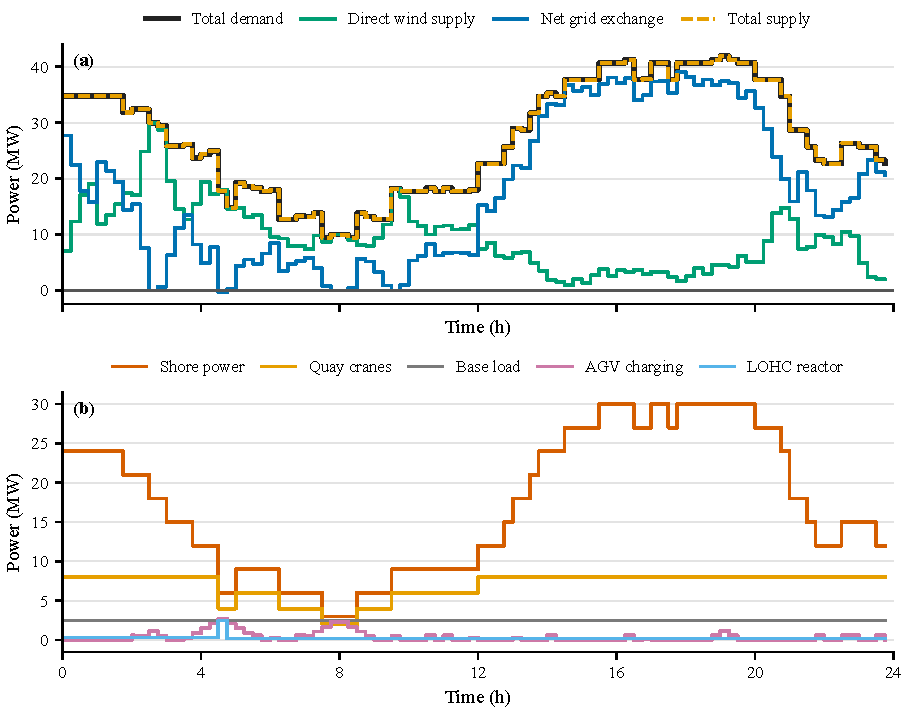
\includegraphics[width=0.98\linewidth]{figures/c1_confirmed_main_budget_20260714/c1_day_ahead_dispatch.pdf}
  \caption{Corrected C1 day-ahead dispatch. Panel (a) verifies the nominal power balance; panel (b) reports the principal port demand components.}
  \label{fig:c1-day-ahead-dispatch}
\end{figure}

% Dedicated AGV/LOHC day-ahead versus intraday comparison.
\begin{figure}[t]
  \centering
  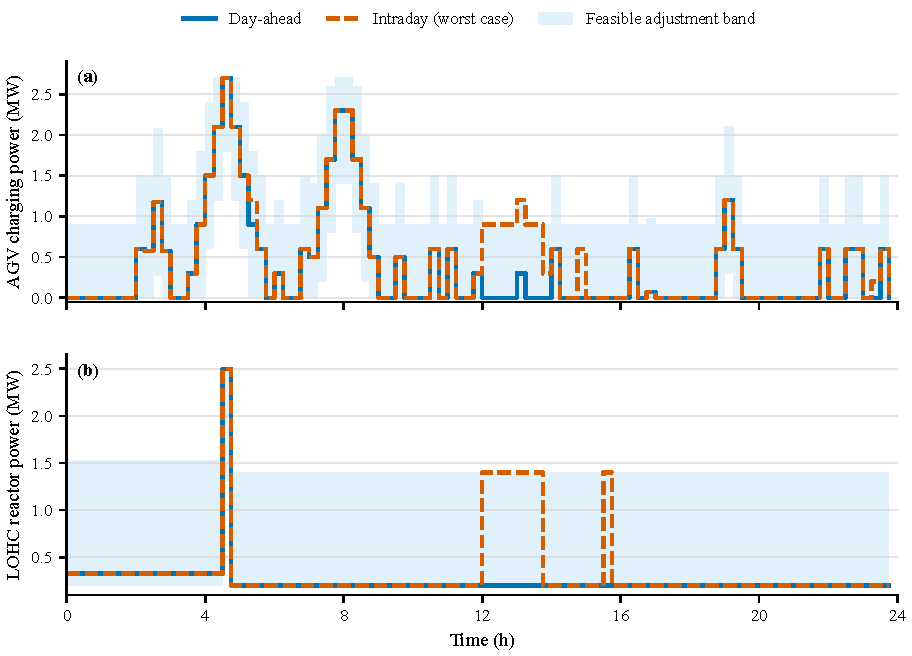
\includegraphics[width=0.98\linewidth]{figures/c1_confirmed_main_budget_20260714/c1_agv_lohc_day_ahead_intraday_comparison.pdf}
  \caption{AGV charging and LOHC reactor powers in the corrected C1 day-ahead schedule and the certified worst-case intraday recourse. The shaded feasible bands correspond to the confirmed 0.9 MW and 1.2 MW adjustment limits, respectively.}
  \label{fig:c1-agv-lohc-day-ahead-intraday}
\end{figure}

% Corrected C1 day-ahead and worst-case real-time equipment powers.
\begin{figure}[t]
  \centering
  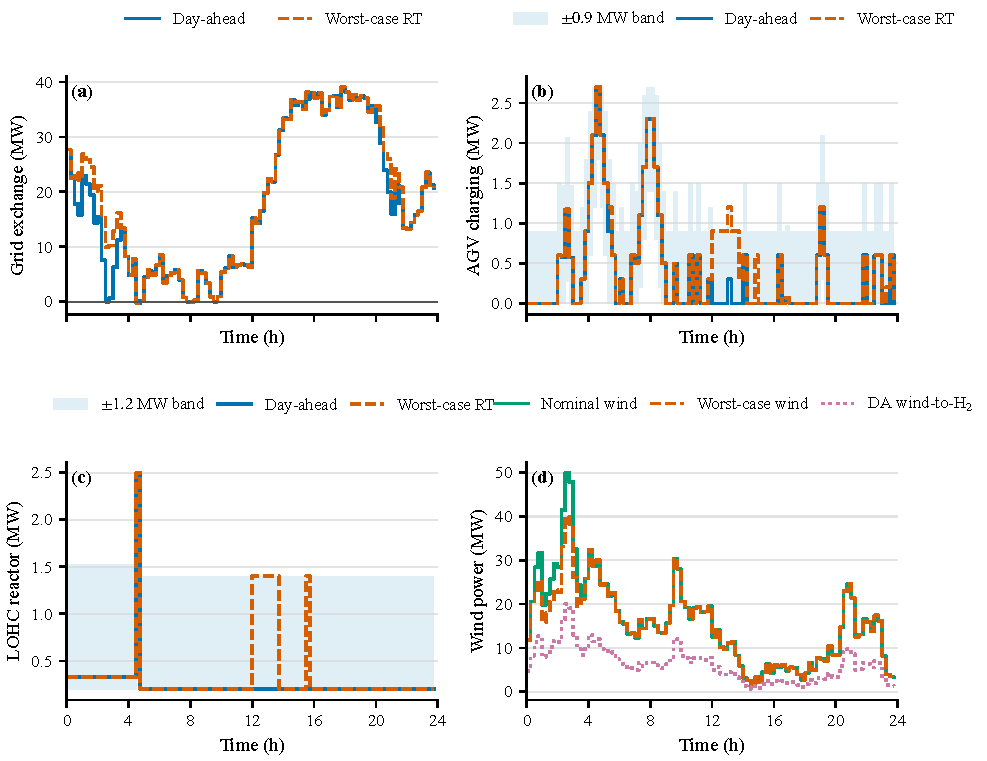
\includegraphics[width=0.98\linewidth]{figures/c1_confirmed_main_budget_20260714/c1_equipment_power_da_vs_worst_rt.pdf}
  \caption{Corrected C1 equipment powers under the day-ahead schedule and the certified worst-case real-time recourse. Shaded regions show the confirmed AGV and LOHC adjustment limits.}
  \label{fig:c1-equipment-power}
\end{figure}
